\documentclass[11pt]{article}
\usepackage{homework}

\classname{364}
\homeworknum{5}


\DeclareMathAlphabet{\mathsfit}{T1}{\sfdefault}{\mddefault}{\sldefault}



\begin{document}

% Environments

\newcommand{\state}[2]{\begin{statement}{#1} #2 \end{statement}}
\newcommand{\prob}[2]{\begin{problem}{#1} #2 \end{problem}}
\newcommand{\subprob}[1]{\begin{subproblem} #1 \end{subproblem}}
\newcommand{\sol}[1]{\begin{solution} #1 \end{solution}}
\newcommand{\fig}[2]{\begin{figure} \centering #2  \label{#1} \end{figure}}

\newcommand{\makebib}{
	\vfill
	\color{black}
	\nocite{*}
	\bibliography{references}{}
	\bibliographystyle{lucas_unsrt}
}
	

% Implication

\newcommand{\qwhere}{\quad \text{where} \quad}
\newcommand{\qimplies}{\quad \implies \quad}
\newcommand{\impliesq}{\implies \quad}



% Brackets

\newcommand{\paren}[1]{\left( #1 \right)}
\newcommand{\brac}[1]{\left[ #1 \right]}
\newcommand{\curly}[1]{\left\{ #1 \right\}}


% Greek

\newcommand{\alp}{\alpha}
\newcommand{\bet}{\beta}
\newcommand{\gam}{\gamma}
\newcommand{\del}{\delta}
\newcommand{\eps}{\epsilon}
\newcommand{\zet}{\zeta}
\newcommand{\tht}{\theta}
\newcommand{\kap}{\kappa}
\newcommand{\lam}{\lambda}
\newcommand{\sig}{\sigma}
\newcommand{\ups}{\upsilon}
\newcommand{\omg}{\omega}

\newcommand{\Gam}{\Gamma}
\newcommand{\Del}{\Delta}
\newcommand{\Tht}{\Theta}
\newcommand{\Lam}{\Lambda}
\newcommand{\Sig}{\Sigma}
\newcommand{\Omg}{\Omega}


% Text

\newcommand{\where}{\text{where }}

% Problem 1

\newcommand{\Hint}{H_\text{int}}
\newcommand{\ddcx}{\dd[3]{x}}
\newcommand{\psib}{\bar{\psi}}

\newcommand{\mh}{m_h}
\newcommand{\mmu}{m_\mu}
\newcommand{\me}{m_e}
\newcommand{\ma}{m_a}

\newcommand{\aexpt}{a_\text{expt.}}
\newcommand{\aQED}{a_\text{QED}}
\renewcommand{\GeV}{\giga\electronvolt}

\newcommand{\gamt}{\gam^5}



\state{Ocean tides~(MCP 25.9)}{\hfix}

\prob{
	Place a local Lorentz frame at the center of Earth, and let $\cEsjk$ be the tidal field there, produced by the Newtonian gravitational fields of the Sun and the Moon.  For simplicity, treat Earth as precisely spherical.  Show that the gravitational acceleration (relative to Earth's center) at some location on or near Earth's surface (radius $r$) is
	\eq{
		\gsj = -\frac{G M}{r^2} \nj - \cEjsk r \nk,
	}
	where $M$ is Earth's mass, and $\nj$ is a unit vector pointing from Earth's center to the location at which $\gsj$ is evaluated.
}



\prob{
	Show that this gravitational acceleration is minus the gradient of the Newtonian potential
	\eq{
		\Phi = -\frac{G M}{r} + \frac{1}{2} \cEsjk r^2 \nj \nk.
	}
}



\prob{
	Consider regions of Earth's oceans that are far from any coast and have ocean depth large compared to the heights of ocean tides.  If Earth were nonrotating, then explain why the analysis of Sec~13.3 predicts that the ocean surface in these regions would be a surface of constant $\Phi$.  Explain why this remains true to good accuracy also for the rotating Earth.
}



\prob{
	Show that in these ocean regions, the Moon creates high tides pointing toward and away from itself and low tides in the transverse directions on Earth; and similarly for the Sun.  Compute the difference between high and low tides produced by the Moon and by the Sun, and the difference of the total tide when the Moon and the Sun are in approximately the same direction in the sky.  Your answers are reasonably accurate for deep-ocean regions far from any coast, but near a coast, the tides are typically larger and sometimes far larger, and they are shifted in phase relative to the positions of the moon and Sun.  Why?
}






\clearpage
\newcommand{\Fab}{F^{\alp \bet}}
\newcommand{\Ua}{U^\alp}
\newcommand{\Usa}{U_\alp}
\newcommand{\Ub}{U^\bet}
\newcommand{\Xa}{X^\alp}
\newcommand{\Xsa}{X_\alp}
\newcommand{\Xb}{X^\bet}
\newcommand{\xap}{x^\alp_p}
\newcommand{\xaq}{x^\alp_q}

\begin{statement}{(Jackson 11.17)}
	The electric and magnetic fields \refeq{fields} of a charge in uniform motion can be obtained from Coulomb's law in the charge's rest frame and the fact that the field strength $\Fab$ is an antisymmetric tensor of rank 2 without considering \emph{explicitly} the Lorentz transformation.  The idea is the following.  For a charge in uniform motion the only relevant variables are the charge's 4-velocity $\Ua$ and the relative coordinate $\Xa = \xap - \xaq$, where $\xap$ and $\xaq$ are the 4-vector coordinates of the observation point and the charge, respectively.  The only antisymmetric tensor that can be formed is $(\Xa \Ub - \Xb \Ua)$.  Thus the electromagnetic field $\Fab$ must be this tensor multiplied by some scalar function of the possible scalar products, $\Xsa \Xa$, $\Xsa \Ua$, $\Usa \Ua$.
\end{statement}

\newcommand{\vbb}{\vb{b}}
\newcommand{\vv}{\vb{v}}
\newcommand{\Eq}{E_1}
\newcommand{\Ew}{E_2}
\newcommand{\Ee}{E_3}
\newcommand{\Bq}{B_1}
\newcommand{\Bw}{B_2}
\newcommand{\Be}{B_3}

\newcommand{\xsq}{x^1}


\begin{figure} \centering
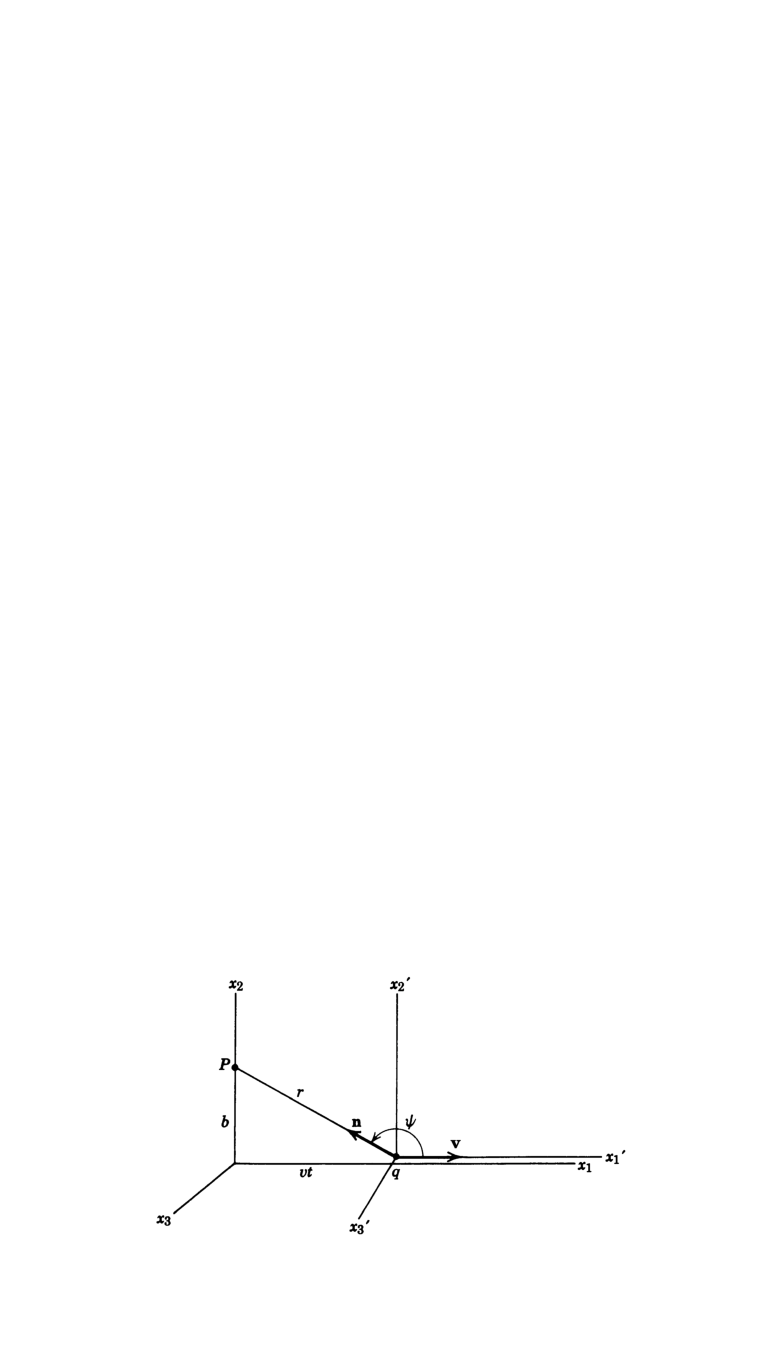
\includegraphics{11-8}
\caption{(Jackson Fig.~11.8) Particle of charge $q$ moving at constant velocity $\vv$ passes an observation point $P$ at impact parameter $b$.}
\label{11.8}
\end{figure}

\begin{problem} \label{2.a}
	For the geometry of Fig.~\ref{11.8} the coordinates of $P$ and $q$ at a common time in $K$ can be written $\xap = (ct, \vbb)$, $\xaq = (ct, \vv t)$, with $\vbb \vdot \vv = 0$.  By considering the general form of $\Fab$ in the rest frame of the charge, show that
	\beqn \label{show2.a}
		\Fab = \frac{q}{c} \frac{\Xa \Ub - \Xb \Ua}{[(\Usa \Xa / c)^2 - \Xsa \Xa]^{3/2}}.
	\eeqn
	Verify that this yields the expressions
	\begin{align} \label{fields}
		\Eq &= \Eq' = -\frac{q \gam v t}{(b^2 + \gam^2 v^2 t^2)^{3/2}}, &
		\Ew &= \gam \Ew' = \frac{\gam q b}{(b^2 + \gam^2 v^2 t^2)^{3/2}}, &
		\Be &= \gam \bet \Ew' = \bet \Ew,
	\end{align}
	with all other components vanishing, in the inertial frame $K$.
\end{problem}


\newcommand{\Fmat}{\mqty[	0 & -\Eq & -\Ew & -\Ee \\
						\Eq & 0 & -\Be & \Bw \\
						\Ew & \Be & 0 & -\Bq \\
						\Ee & -\Bw & \Bq & 0 ]}
\newcommand{\Fpab}{{F'}^{\alp\bet}}
\newcommand{\rp}{{r'}}
\newcommand{\tLam}{\tilde{\Lam}}
\newcommand{\Lammat}{\mqty[\gam & \gam \beta & 0 & 0 \\	
						\gam \beta & \gam & 0 & 0 \\
						0 & 0 & 1 & 0 \\
						0 & 0 & 0 & 1 ]}

\begin{solution}
	From Jackson~(11.137),
	\beqn \label{F}
		\Fab = \Fmat,
	\eeqn
	and from the equation immediately preceding Jackson~(11.151),
	\begin{align*}
		\Eq' &= -\frac{q v t'}{\rp^3}, &
		\Ew' &= \frac{q b}{\rp^3}, &
		\Ee' &= 0, &
		\Bq' &= 0, &
		\Bw' &= 0, &
		\Be' &= 0,
	\end{align*}
	in the rest frame of the charge for the geometry in Fig.~\ref{1}.  Here, $r' = \sqrt{b^2 + v^2 {t'}^2}$.  Then, in $K'$,
	\beqn \label{thing2.1b}
		\Fpab = \frac{q}{(b^2 + v^2 {t'}^2)^{3/2}}
			\mqty[0 & v t' & -b & 0 \\
				-v t' & 0 & 0 & 0 \\
				b & 0 & 0 & 0 \\
				0 & 0 & 0 & 0 ].
	\eeqn
	Now we will boost into the frame $K$.  From Jackson~(11.147), $F' = \Lam F \tLam$, although we need $F = \Lam F' \tLam$, where we boost in the direction opposite the particle's motion.  According to Jackson~(11.113), the Lorentz boost in the $-x'$ direction is
	\beqn \label{Lam2}
		\Lam = \Lammat.
	\eeqn
	Then
	\begin{align*}
		\Fab &= \frac{q}{(b^2 + v^2 {t'}^2)^{3/2}} \Lammat
			\mqty[ 0 & v t' & -b & 0 \\
				-v t' & 0 & 0 & 0 \\
				b & 0 & 0 & 0 \\
				0 & 0 & 0 & 0 ]
			\Lammat \\
		&= \frac{q}{(b^2 + v^2 {t'}^2)^{3/2}}
			\mqty[ -\gam \bet v t' & \gam v t' & -\gam b & 0 \\
				-\gam v t' & \gam \bet v t' & -\gam \bet b & 0 \\
				b & 0 & 0 & 0 \\
				0 & 0 & 0 & 0 ]
			\Lammat
		= \frac{q}{(b^2 + v^2 {t'}^2)^{3/2}}
			\mqty[ 0 & v t' & -\gam b & 0 \\
				-v t' & 0 & -\gam \bet b & 0 \\
				\gam b & \gam \bet b & 0 & 0 \\
				0 & 0 & 0 & 1 ].
	\end{align*}
	From \refeq{lorentz}, $t' = \gam t$ since $x = 0$.  Finally,
	\beqn \label{thing2.1}
		\Fab = \frac{\gam q}{(b^2 + \gam^2 v^2 t^2)^{3/2}} 
			\mqty[0 & v t & -b & 0 \\
				-v t & 0 & -v b / c & 0 \\
				b & v b / c & 0 & 0 \\
				0 & 0 & 0 & 0 ].
	\eeqn
	
	Now we will begin from \refeq{show2.a} and find $\Fab$ directly in $K$.  In accordance with Fig.~\ref{11.8},
	\begin{align*}
		\Xa &= (0, \vbb - \vv t) = (0, -v t, b, 0), &
		\Ua &= \gam (c, \vv) = \gam (c, v, 0, 0),
	\end{align*}
	and so
	\beq
		\Xa \Ub - \Xb \Ua = \gam
			\mqty[ 0 & 0 & 0 & 0 \\
				-c v t & -v^2 t & 0 & 0 \\
				c b & v b & 0 & 0 \\
				0 & 0 & 0 & 0 ]
		- \gam
			\mqty[ 0 & -c v t & c b & 0 \\
				0 & -v^2 t & v b & 0 \\
				0 & 0 & 0 & 0 \\
				0 & 0 & 0 & 0 ]
		= \gam
			\mqty[0 & c v t & - c b & 0 \\
				-c v t & 0 & -v b & 0 \\
				c b & v b & 0 & 0 \\
				0 & 0 & 0 & 0 ].
	\eeq
	Additionally,
	\begin{align*}
		\Usa \Xa &= \gam \mqty[ c & -v & 0 & 0 ] \mqty[ 0 \\ -v t \\ b \\ 0 ]
		= \gam v^2 t, &
		\Xsa \Xa &= \mqty[ 0 & vt & -b & 0 ] \mqty[ 0 \\ -v t \\ b \\ 0 ]
		= -v^2 t^2 - b^2.
	\end{align*}
	Then, applying \refeq{show2.a},
	\beq
		\Fab = \frac{\gam q}{(\gam^2 v^4 t^2 / c^2 + v^2 t^2 + b^2)^{3/2}}
			\mqty[0 & v t & -b & 0 \\
				-v t & 0 & -v b / c & 0 \\
				b & v b / c & 0 & 0 \\
				0 & 0 & 0 & 0 ].
	\eeq
	Note that
	\beq
		v^2 t^2 + \frac{\gam^2 v^4 t^2}{c^2} = v^2 t^2 \left( 1 + \gam^2 \frac{v^2}{c^2} \right)
		= v^2 t^2 \left( 1 + \frac{\bet^2}{1 - \bet^2} \right)
		= v^2 t^2 \frac{1 - \bet^2 + \bet^2}{1 - \bet^2}
		= \gam^2 v^2 t^2,
	\eeq
	so we have again arrived at \refeq{thing2.1}.  Thus, we have proven \refeq{show2.a}.
	
	In addition, comparing \refeq{thing2.1} with \refeq{F}, we see that
	\begin{align*}
		\Eq &= -\frac{q \gam v t}{(b^2 + \gam^2 v^2 t^2)^{3/2}}, &
		\Ew &= \frac{\gam q b}{(b^2 + \gam^2 v^2 t^2)^{3/2}}, &
		\Be &= \frac{\gam \bet q b}{(b^2 + \gam^2 v^2 t^2)^{3/2}} = \bet \Ew.
	\end{align*}
	Comparing \refeq{thing2.1b} with \refeq{F} as well, and making the substitution $t' = \gam t$, yields
	\begin{align*}
		\Eq' &= -\frac{q \gam v t}{(b^2 + \gam^2 v^2 t^2)^{3/2}}, &
		\Ew' &= \frac{q b}{(b^2 + \gam^2 v^2 t^2)^{3/2}},
	\end{align*}
	so we have also verified \refeq{fields}. \qed
\end{solution}


\newcommand{\xpap}{{x'}^\alp_p}
\newcommand{\xpaq}{{x'}^\alp_q}
\newcommand{\Ya}{Y^\alp}
\newcommand{\Ysa}{Y_\alp}
\newcommand{\Yb}{Y^\bet}
\newcommand{\Ypa}{{Y'}^\alp}

\begin{problem}
	Repeat the calculation, using as the starting point the common-time coordinates in the rest frame, ${\xpap = (ct', \vbb - \vv t')}$ and $\xpaq = (ct', 0)$.  Show that
	\beqn \label{show2.b}
		\Fab = \frac{q}{c} \frac{\Ya \Ub - \Yb \Ua}{(- \Ysa \Ya)^{3/2}},
	\eeqn
	where $\Ypa = \xpap - \xpaq$.  Verify that the fields are the same as in \ref{2.a}.  Note that to obtain the results of \refeq{fields} it is necessary to use the time $t$ of the observation point $P$ in $K$ as the time parameter.
\end{problem}

\newcommand{\Ypsa}{{Y'}_\alp}
\newcommand{\Ypb}{{Y'}^\bet}
\newcommand{\Upa}{{U'}^\alp}
\newcommand{\Upb}{{U'}^\bet}
\newcommand{\vo}{\mathbf{0}}
\newcommand{\tp}{{t'}}

\begin{solution}
	Firstly, note that
	\begin{align*}
		\Ypa &= (0, \vbb - \vv t') = (0, -v t', b, 0), &
		\Upa &= (c, \vo) = (c, 0, 0, 0),
	\end{align*}
	Then
	\beq
		\Ypa \Upb - \Ypb \Upa = c
			\mqty[ 0 & 0 & 0 & 0 \\
				-v t' & 0 & 0 & 0 \\
				b & 0 & 0 & 0 \\
				0 & 0 & 0 & 0 ]
		- c
			\mqty[ 0 & -v t' & b & 0 \\
				0 & 0 & 0 & 0 \\
				0 & 0 & 0 & 0 \\
				0 & 0 & 0 & 0 ]
		= c
			\mqty[ 0 & v t' & -b & 0 \\
				-v t' & 0 & 0 & 0 \\
				b & 0 & 0 & 0 \\
				0 & 0 & 0 & 0 ],
	\eeq
	and
	\beq
		\Ypsa \Ypa = \mqty[ 0 & v t' & -b & 0 ] \mqty[ 0 \\ -v t' \\ b \\ 0 ] = -v^2 \tp^2 - b^2,
	\eeq
	so, from \refeq{show2.b}, in $K'$ we have
	\beq
		\Fpab = \frac{q}{(b^2 + v^2 \tp^2)^{3/2}}
			\mqty[ 0 & v t' & -b & 0 \\
				-v t' & 0 & 0 & 0 \\
				b & 0 & 0 & 0 \\
				0 & 0 & 0 & 0 ],
	\eeq
	which is identical to \refeq{thing2.1b}.  We know that boosting into $K$ yields \refeq{thing2.1}.
	
	Now we will find $\Fab$ directly in $K$ by boosting $\Ypa$ and $\Upa$.  From Jackson~(11.84), $x' = \Lam x$ (where $x$ represents $x^\alp$), and we once again use $\Lam$ given by \refeq{Lam2} to perform $x = \Lam x'$.  We obtain
	\begin{align*}
		Y &= \Lam Y'
		= \Lammat \mqty[ 0 \\ -v t' \\ b \\ 0]
		= \mqty[ -\gam \bet v t' \\ -\gam v t' \\ b \\ 0 ], &
		U &= \Lam U'
		= \Lammat \mqty[ c \\ 0 \\ 0 \\ 0 ]
		= \gam c \mqty[ 1 \\ \bet \\ 0 \\ 0 ].
	\end{align*}
	Then
	\beq
		\Ya \Ub - \Yb \Ua = \gam c
			\mqty[ -\gam \bet v t' & -\gam \bet^2 v t' & 0 & 0 \\
				-\gam v t' & -\gam \bet v t' & 0 & 0 \\
				b & \bet b & 0 & 0 \\
				0 & 0 & 0 & 0 ]
			- \gam c
			\mqty[ -\gam \bet v t' & -\gam v t' & b & 0 \\
				-\gam \bet^2 v t' & -\gam \bet v t' & \bet b & 0 \\
				0 & 0 & 0 & 0 \\
				0 & 0 & 0 & 0 ]
		= c
			\mqty[ 0 & v t' & -\gam b & 0 \\
				-v t' & 0 & -\gam \bet b & 0 \\
				\gam b & \gam \bet b & 0 & 0 \\
				0 & 0 & 0 & 0 ],
	\eeq
	and
	\beq
		\Ysa \Ya = \mqty[ -\gam \bet v t' & \gam v t' & -b & 0] \mqty[ -\gam \bet v t' \\ -\gam v t' \\ b \\ 0 ]
		= \gam^2 \bet^2 v^2 \tp^2 - \gam^2 v^2 \tp^2 - b^2
		= -v^2 \tp^2 - b^2.
	\eeq
	Making these substitutions into \refeq{show2.b}, and using $t' = \gam t$,
	\beq
		\Fab = \frac{q}{(b^2 + v^2 \tp^2)^{3/2}}
			\mqty[ 0 & v t' & -\gam b & 0 \\
				-v t' & 0 & -\gam v b / c & 0 \\
				\gam b & \gam v b / c & 0 & 0 \\
				0 & 0 & 0 & 0 ]
		= \frac{\gam q}{(b^2 + \gam^2 v^2 t^2)^{3/2}}
			\mqty[ 0 & v t & -b & 0 \\
				-v t & 0 & -v b / c & 0 \\
				b & v b / c & 0 & 0 \\
				0 & 0 & 0 & 0 ],
	\eeq
	which is identical to \refeq{thing2.1}, and therefore gives the fields from \refeq{fields} as in \ref{2.a}.  Thus, we have proven \refeq{show2.b}. \qed
\end{solution}


\newcommand{\Za}{Z^\alp}
\newcommand{\Zsa}{Z_\alp}
\newcommand{\Zb}{Z^\bet}
\newcommand{\vbet}{\boldsymbol{\beta}}

\begin{problem}
	Finally, consider the coordinate $\xap = (ct, \vbb)$ and the ``retarded-time'' coordinate $\xaq = [ct - R, \vbet(ct - R)]$ where $R$ is the distance between $P$ and $q$ at the retarded time.  Define the difference as $\Za = [R, \vbb - \vbet(ct - R)]$.  Show that in terms of $\Za$ and $\Ua$ the field is
	\beqn \label{show2.c}
		\Fab = \frac{q}{c} \frac{\Za \Ub - \Zb \Ua}{(\Usa \Za / c)^3}.
	\eeqn
\end{problem}
\vfix

\begin{solution}
	Referring to Fig~\ref{11.8},
	\begin{align*}
		\Za &= (R, \vbb - \vv t + \vv R / c) = [R, -v (t - R / c), b, 0], &
		\Ua &= \gam (c, \vv) = \gam (c, v, 0, 0).
	\end{align*}
	Then
	\begin{align*}
		\Za\Ub - \Zb \Ua &= \gam
			\mqty[c R & R v & 0 & 0 \\
				-v (c t - R) & -v^2 (t - R / c) & 0 & 0 \\
				c b & b v & 0 & 0 \\
				0 & 0 & 0 & 0 ]
			- \gam
			\mqty[ c R & -v (c t - R) & c b & 0 \\
				R v & -v^2 (t - R / c) & b v & 0 \\
				0 & 0 & 0 & 0 \\
				0 & 0 & 0 & 0 ] \\
		&= \gam c
			\mqty[0 & v t & -b & 0 \\
				-v t & 0 & -v b / c & 0 \\
				b & v b / c & 0 & 0 \\
				0 & 0 & 0 & 0 ],
	\end{align*}
	and
	\beq
		\Usa \Za = \gam \mqty[ c & -v & 0 & 0 ] \mqty[ R \\ -v (t - R / c) \\ b \\ 0 ]
		= \gam cR + \gam v^2(t - R/c),
	\eeq
	so
	\beq
		\frac{\Usa \Za}{c} = \gam R + \gam \bet^2 c t - \gam \bet^2 R
		= (1 - \bet^2) \gam R + \gam \bet^2 c t
		= \frac{R}{\gam} + \gam \bet^2 c t.
	\eeq
	
	Note that $\xap$ and $\xaq$, as they are defined here, have lightlike separation since $R / c$ is, by definition, the time it takes light to travel from $\xaq$ to $\xap$.  Then
	\beq
		0 = \Zsa \Za
		= \mqty[ R & v (t - R / c) & -b & 0 ] \mqty[ R \\ -v (t - R / c) \\ b \\ 0 ]
		= R^2 - v^2 (t - R / c)^2 - b^2,
	\eeq
	which implies
	\beq
		R^2 = b^2 + v^2 (t - R / c)^2.
	\eeq
	This is corroborated by the geometry of Fig.~\ref{11.8}, since $t - R / c$ is the retarded time.  Then, referring to the denominator of \refeq{thing2.1}, we find
	\begin{align*}
		b^2 + \gam^2 v^2 t^2 &= R^2 - v^2 (t - R / c)^2 + \gam^2 v^2 t^2
		= R^2 - \bet^2  (c^2 t^2 - 2 R c t + R^2) + \gam^2 \bet^2 c^2 t^2 \\
		&= (1 - \bet^2) R^2 + 2 R \bet^2 c t + (\gam^2 - 1) \bet^2 c^2 t^2
		= \frac{R^2}{\gam^2} + 2 R \bet^2 c t + \gam^2 \bet^4 c^2 t^2
		= \left( \frac{R}{\gam} + \gam \bet^2 c t \right)^2 \\
		&= \left( \frac{\Usa \Za}{c} \right)^2.
	\end{align*}
	In summary, we have found
	\beq
		\Fab = \frac{\gam q}{(b^2 + \gam^2 v^2 t^2)^{3/2}}
			\mqty[0 & v t & -b & 0 \\
				-v t & 0 & -v b / c & 0 \\
				b & v b / c & 0 & 0 \\
				0 & 0 & 0 & 0 ],
	\eeq
	which is identical to \refeq{thing2.1}.  Thus, we have proven \refeq{show2.c}. \qed
\end{solution}






\clearpage
\state{Weyl curvature tensor~(MCP 25.12)}{
	Show that the Weyl curvature tensor~(25.48) has vanishing contraction on all its slots and has the same symmetries as Riemann: Eqs.~(25.45).  From these properties, show that Weyl has just 10 independent components.  Write the Riemann tensor in terms of the Weyl tensor, the Ricci tensor, and the scalar curvature.
}

\sol{
	MCP~(25.48) is
	\eqn{weyl}{
		\fv{C}{\mu \nu}{\rho \sig} = \fv{R}{\mu \nu}{\rho \sig} - 2 \fv{\sg}{[ \mu}{[ \rho} \fv{R}{\nu ]}{\sig ]} + \frac{1}{3} \fv{\sg}{[ \mu}{[ \rho} \fv{\sg}{\nu ]}{\sig ]} R,
	}
	where the square brackets denote antisymmetrization, $A_{[ \alp \bet ]} = (A_{\alp \bet} - A_{\bet \alp}) / 2$, and $R = \fv{R}{\alp}{\alp}$.  Lowering the indices and expanding out the antisymmetrizations gives us
	\aln{
		C_{\mu \nu \rho \sig} &= R_{\mu \nu \rho \sig} - \paren{ \sg_{\mu \ [ \rho} R_{\nu \ \sig ]} - \sg_{\nu \ [ \rho} R_{\mu \ \sig ]} } + \frac{1}{6} \paren{ \sg_{\mu \ [ \rho} \sg_{\nu \ \sig ]} - \sg_{\nu \ [ \rho} \sg_{\mu \ \sig ]} } R \notag \\
		&= R_{\mu \nu \rho \sig} - \frac{1}{2} \paren{ \sg_{\mu \rho} R_{\nu \sig} - \sg_{\mu \sig} R_{\nu \rho} - \sg_{\nu \rho} R_{\mu \sig} + \sg_{\nu \sig} R_{\mu \rho} } + \frac{1}{12} \paren{ \sg_{\mu \rho} \sg_{\nu \sig} - \sg_{\mu \sig} \sg_{\nu \rho} - \sg_{\nu \rho} \sg_{\mu \sig} + \sg_{\nu \sig} \sg_{\mu \rho} } R. \label{lowC}
	}
	
	We begin by interchanging indices since it makes the other proofs easier.  Interchanging the first two indices,
	\al{
		C_{\nu \mu \rho \sig} &= R_{\nu \mu \rho \sig} - \frac{1}{2} \paren{ \sg_{\nu \rho} R_{\mu \sig} - \sg_{\nu \sig} R_{\mu \rho} - \sg_{\mu \rho} R_{\nu \sig} + \sg_{\mu \sig} R_{\nu \rho} } + \frac{1}{12} \paren{ \sg_{\nu \rho} \sg_{\mu \sig} - \sg_{\nu \sig} \sg_{\mu \rho} - \sg_{\mu \rho} \sg_{\nu \sig} + \sg_{\mu \sig} \sg_{\nu \rho} } R \\
		&= -\brac{ R_{\mu \nu \rho \sig} - \frac{1}{2} \paren{ \sg_{\mu \rho} R_{\nu \sig} - \sg_{\mu \sig} R_{\nu \rho} - \sg_{\nu \rho} R_{\mu \sig} + \sg_{\nu \sig} R_{\mu \rho} } + \frac{1}{12} \paren{ \sg_{\mu \rho} \sg_{\nu \sig} - \sg_{\mu \sig} \sg_{\nu \rho} - \sg_{\nu \rho} \sg_{\mu \sig} + \sg_{\nu \sig} \sg_{\mu \rho} } R } \\
		&= - C_{\mu \nu \rho \sig},
	}
	where we have used $R_{\alp \bet \gam \del} = -R_{\bet \alp \gam \del}$ from MCP~(25.45a).
	
	Interchanging the last two indices,
	\al{
		C_{\mu \nu \sig \rho} &= R_{\mu \nu \sig \rho} - \frac{1}{2} \paren{ \sg_{\mu \sig} R_{\nu \rho} - \sg_{\mu \rho} R_{\nu \sig} - \sg_{\nu \sig} R_{\mu \rho} + \sg_{\nu \rho} R_{\mu \sig} } + \frac{1}{12} \paren{ \sg_{\mu \sig} \sg_{\nu \rho} - \sg_{\mu \rho} \sg_{\nu \sig} - \sg_{\nu \sig} \sg_{\mu \rho} + \sg_{\nu \rho} \sg_{\mu \sig} } R \\
		&= -\brac{ R_{\mu \nu \rho \sig} - \frac{1}{2} \paren{ \sg_{\mu \rho} R_{\nu \sig} - \sg_{\mu \sig} R_{\nu \rho} - \sg_{\nu \rho} R_{\mu \sig} + \sg_{\nu \sig} R_{\mu \rho} } + \frac{1}{12} \paren{ \sg_{\mu \rho} \sg_{\nu \sig} - \sg_{\mu \sig} \sg_{\nu \rho} - \sg_{\nu \rho} \sg_{\mu \sig} + \sg_{\nu \sig} \sg_{\mu \rho} } R } \\
		&= - \fv{C}{\mu \nu}{\rho \sig},
	}
	where we have used $R_{\alp \bet \gam \del} = -R_{\alp \bet \del \gam}$ from MCP~(25.45a).
	
	Interchanging the first and second pair of indices,
	\al{
		C_{\rho \sig \mu \nu} &= R_{\rho \sig \mu \nu} - \frac{1}{2} \paren{ \sg_{\rho \mu} R_{\sig \nu} - \sg_{\rho \nu} R_{\sig \mu} - \sg_{\sig \mu} R_{\rho \nu} + \sg_{\sig \nu} R_{\rho \mu} } + \frac{1}{12} \paren{ \sg_{\rho \mu} \sg_{\sig \nu} - \sg_{\rho \nu} \sg_{\sig \mu} - \sg_{\sig \mu} \sg_{\rho \nu} + \sg_{\sig \nu} \sg_{\rho \mu} } R \\
		&= R_{\mu \nu \rho \sig} - \frac{1}{2} \paren{ \sg_{\mu \rho} R_{\nu \sig} - \sg_{\mu \sig} R_{\nu \rho} - \sg_{\nu \rho} R_{\mu \sig} + \sg_{\nu \sig} R_{\mu \rho} } + \frac{1}{12} \paren{ \sg_{\mu \rho} \sg_{\nu \sig} - \sg_{\mu \sig} \sg_{\nu \rho} - \sg_{\nu \rho} \sg_{\mu \sig} + \sg_{\nu \sig} \sg_{\mu \rho} } R \\
		&= \fv{C}{\mu \nu}{\rho \sig},
	}
	where we have used the symmetry of the metric, $\fv{\sg}{\mu}{\nu} = \fv{\sg}{\nu}{\mu}$, and $R_{\alp \bet \gam \del} = +R_{\gam \del \alp \bet}$ from MCP~(25.45a).

	Note also that
	\al{
		C_{\mu \rho \sig \nu} &= R_{\mu \rho \sig \nu} - \frac{1}{2} \paren{ \sg_{\mu \sig} R_{\rho \nu} - \sg_{\mu \nu} R_{\rho \sig} - \sg_{\rho \sig} R_{\mu \nu} + \sg_{\rho \nu} R_{\mu \sig} } + \frac{1}{12} \paren{ \sg_{\mu \sig} \sg_{\rho \nu} - \sg_{\mu \nu} \sg_{\rho \sig} - \sg_{\rho \sig} \sg_{\mu \nu} + \sg_{\rho \nu} \sg_{\mu \sig} } R, \\
		%
		C_{\mu \sig \nu \rho} &= R_{\mu \sig \nu \rho} - \frac{1}{2} \paren{ \sg_{\mu \nu} R_{\sig \rho} - \sg_{\mu \rho} R_{\sig \nu} - \sg_{\sig \nu} R_{\mu \rho} + \sg_{\sig \rho} R_{\mu \nu} } + \frac{1}{12} \paren{ \sg_{\mu \nu} \sg_{\sig \rho} - \sg_{\mu \rho} \sg_{\sig \nu} - \sg_{\sig \nu} \sg_{\mu \rho} + \sg_{\sig \rho} \sg_{\mu \nu} } R.
	}
	Then for the equivalent to MCP~(25.45b),
	\al{
		C_{\mu \nu \rho \sig} + C_{\mu \rho \sig \nu} + C_{\mu \sig \nu \rho}
		&= R_{\mu \nu \rho \sig} + R_{\mu \rho \sig \nu} + R_{\mu \sig \nu \rho} - \frac{1}{2} \paren{ \sg_{\mu \rho} R_{\nu \sig} - \sg_{\mu \sig} R_{\nu \rho} - \sg_{\nu \rho} R_{\mu \sig} + \sg_{\nu \sig} R_{\mu \rho} } \\
		&\hspace{5em} \phantom{=} - \frac{1}{2} \paren{ \sg_{\mu \sig} R_{\rho \nu} - \sg_{\mu \nu} R_{\rho \sig} - \sg_{\rho \sig} R_{\mu \nu} + \sg_{\rho \nu} R_{\mu \sig} } \\
		&\hspace{5em} \phantom{=} - \frac{1}{2} \paren{ \sg_{\mu \nu} R_{\sig \rho} - \sg_{\mu \rho} R_{\sig \nu} - \sg_{\sig \nu} R_{\mu \rho} + \sg_{\sig \rho} R_{\mu \nu} } \\
		&\hspace{5em} \phantom{=} + \frac{1}{12} \paren{ \sg_{\mu \rho} \sg_{\nu \sig} - \sg_{\mu \sig} \sg_{\nu \rho} - \sg_{\nu \rho} \sg_{\mu \sig} + \sg_{\nu \sig} \sg_{\mu \rho} } R \\
		&\hspace{5em} \phantom{=} + \frac{1}{12} \paren{ \sg_{\mu \sig} \sg_{\rho \nu} - \sg_{\mu \nu} \sg_{\rho \sig} - \sg_{\rho \sig} \sg_{\mu \nu} + \sg_{\rho \nu} \sg_{\mu \sig} } R \\
		&\hspace{5em} \phantom{=} + \frac{1}{12} \paren{ \sg_{\mu \nu} \sg_{\sig \rho} - \sg_{\mu \rho} \sg_{\sig \nu} - \sg_{\sig \nu} \sg_{\mu \rho} + \sg_{\sig \rho} \sg_{\mu \nu} } R \\
		&= 0,
	}
	where we have used $R_{\alp \bet \gam \del} + R_{\alp \gam \del \bet} + R_{\alp \del \bet \gam} = 0$ from MCP~(25.45b), and the symmetry of the metric tensor.  Thus we have shown that the Weyl curvature tensor has the same symmetries as Riemann in MCP~(25.45): \vfix
	\ans{\aln{ \label{Csymm}
		C_{\nu \mu \rho \sig} &= -C_{\mu \nu \rho \sig}, &
		C_{\mu \nu \sig \rho} &= -C_{\mu \nu \rho \sig}, &
		C_{\rho \sig \mu \nu} &= +C_{\mu \nu \rho \sig}, &
		C_{\mu \nu \rho \sig} + C_{\mu \rho \sig \nu} + C_{\mu \sig \nu \rho} &= 0.
	}}%
	Now for the contractions.  Contracting the indices within each pair,
	\aln{ \label{thingy2}
		\sg^{\mu \nu} C_{\mu \nu \rho \sig} &= \sfvt{C}{\mu}{\mu}{\rho \sig}
		= -\sfvt{C}{\mu}{\mu}{\rho \sig}
		= 0, &
		%
		\sg^{\rho \sig} C_{\mu \nu \rho \sig} &= \sfv{C}{\mu \nu \rho}{\rho}
		= -\sfv{C}{\mu \nu \rho}{\rho}
		= 0,
	}
	where we have used $C_{\nu \mu \rho \sig} = -C_{\mu \nu \rho \sig}$ and our ability to swap covariant and contravariant for summed indices.
	
	Contracting the first and third indices,
	\al{
		\sg^{\mu \rho} C_{\mu \nu \rho \sig} &= \sg^{\mu \rho} \brac{ R_{\mu \nu \rho \sig} - \frac{1}{2} \paren{ \sg_{\mu \rho} R_{\nu \sig} - \sg_{\mu \sig} R_{\nu \rho} - \sg_{\nu \rho} R_{\mu \sig} + \sg_{\nu \sig} R_{\mu \rho} } + \frac{1}{12} \paren{ \sg_{\mu \rho} \sg_{\nu \sig} - \sg_{\mu \sig} \sg_{\nu \rho} - \sg_{\nu \rho} \sg_{\mu \sig} + \sg_{\nu \sig} \sg_{\mu \rho} } R } \\
		&= \sfvt{R}{\mu \nu}{\mu}{\sig} - \frac{1}{2} \paren{ \sfv{\sg}{\mu}{\mu} R_{\nu \sig} - \sg_{\mu \sig} \sfv{R}{\nu}{\mu} - \sfv{\sg}{\nu}{\mu} R_{\mu \sig} + \sg_{\nu \sig} \sfv{R}{\mu}{\mu} } + \frac{1}{12} \paren{ \sfv{\sg}{\mu}{\mu} \sg_{\nu \sig} - \sg_{\mu \sig} \sfv{\sg}{\nu}{\mu} - \sfv{\sg}{\nu}{\mu} \sg_{\mu \sig} + \sg_{\nu \sig} \sfv{\sg}{\mu}{\mu} } R \\
		&= R_{\nu \sig} - \frac{1}{2} \paren{ 4 R_{\nu \sig} - R_{\nu \sig} - R_{\nu \sig} + \sg_{\nu \sig} R } + \frac{1}{12} \paren{ 4 \sg_{\nu \sig} - \sg_{\nu \sig} - \sg_{\nu \sig} + 4 \sg_{\nu \sig} } R \\
		&= R_{\nu \sig} - R_{\nu \sig} - \frac{1}{2} \sg_{\nu \sig} R + \frac{1}{2} \sg_{\nu \sig} R \\
		&= 0,
	}
	where we have used MCP~(24.10), $\sg^{\mu \bet} \sg_{\bet \nu} = \fv{\del}{\mu}{\nu}$, to find $\fv{\sg}{\mu}{\mu} = 4$.  Then, using Eq.~\refeq{Csymm}, we have
	\eq{
		0 = \sfvt{C}{\mu \nu}{\mu}{\sig}
		= -\sfv{C}{\mu \nu \sig}{\mu}
		= -\sfvt{C}{\nu \mu}{\mu}{\sig}
		= \sfv{C}{\nu \mu \sig}{\mu}.
	}
	Rewriting these as contractions, and incorporating our results in Eq.~\refeq{thingy2}, we have shown
	\eq{
		\ans{ 0 = \sg^{\mu \nu} C_{\mu \nu \rho \sig}
		= \sg^{\mu \rho} C_{\mu \nu \rho \sig}
		= \sg^{\mu \sig} C_{\mu \nu \rho \sig}
		= \sg^{\nu \rho} C_{\mu \nu \rho \sig}
		= \sg^{\nu \sig} C_{\mu \nu \rho \sig}
		= \sg^{\rho \sig} C_{\mu \nu \rho \sig}; }
	}
	that is, the Weyl curvature tensor has vanishing contraction on all its slots.
	
	To show that Weyl has just 10 independent components, we refer to the discussion at the end of Lecture~11.  If there were no symmetries, in $n = 4$ spacetime dimensions $C_{\alp \bet \gam \del}$ would have $n^4 = 4^4$ independent components.  Each symmetry gives rise to some number of independent components:
	\al{
		\alp \lrarrow \bet \antisymmetry &\qimplies \frac{n (n - 1)}{2} = 6 \components, \\
		\gam \lrarrow \del \antisymmetry &\qimplies \frac{n (n - 1)}{2} = 6 \components, \\
		\alp \bet \lrarrow \gam \del \symmetry &\qimplies \text{components reduced by } \frac{1}{2}.
	}
	Combining the three (anti)symmetries, we have a total of
	\eq{
		\paren{ \frac{n (n - 1)}{2} } \paren{ \frac{n (n - 1)}{2} + 1 } \frac{1}{2} = 21 \components.
	}
	Now we account for the constraints imposed by $C_{\mu \nu \rho \sig} + C_{\mu \rho \sig \nu} + C_{\mu \sig \nu \rho} = 0$.  This expression is redundant if any of the indices are the same; for example,
	\eq{
		C_{\mu \mu \rho \sig} + C_{\mu \rho \sig \mu} + C_{\mu \sig \mu \rho}
		= 0 + C_{\sig \mu \mu \rho} + C_{\mu \sig \mu \rho}
		= C_{\sig \mu \mu \rho} - C_{\sig \mu \mu \rho}
		= 0,
	}
	which we already knew from the other symmetries.  Since there are four indices, this requirement gives us
	\eq{
		{ n \choose 4 } = 1 \text{ constraint}.
	}
	Finally we account for the constraints imposed by the vanishing contractions.  After accounting for the (anti)symmetries, we are left with two unique vanishing contractions, which impose
	\eq{
		\frac{n (n + 1)}{2} = 10 \constraints.
	}
	\hl{this probably is wrong but eh}
	
	Finally, we find the number of independent components by
	\eq{
		N_\text{components} - N_\text{constraints} = 21 - (1 + 10) = \ans{ 10 \text{ independent components} }
	}
	as we wanted to show. \qed
	
	\hl{general form of 25.48?}
}






\clearpage
\state{Degenerate Bose gas}{\hfix}

%
%	4.1
%

\prob{}{
	The chemical potential of the degenerate Bose gas vanishes below $\Ts$ (the critical temperature of the BEC).  Find its temperature dependence at temperatures slightly above $\Ts$.
}

\sol{
	In three dimensions, the energy distribution of a Bose gas is~\cite[p.~149]{Landau}
	\eqn{ddNeps}{
		\ddNeps = \frac{g V}{\pi^2 \hbar^3} \sqrt{\frac{m^3}{2}} \frac{\sqrt{\eps}}{e^{(\eps - \mu) / T} - 1} \ddeps.
	}
	Integrating over all energies, we find the total number of molecules~\cite[p.~149]{Landau}.  This gives an expression relating the chemical potential $\mu$ and the density $\nb$~\cite[p.~159]{Landau}:
	\eqn{nb}{
		\nb = \frac{g}{\pi^2 \hbar^3} \sqrt{\frac{m^3}{2}} \intoi \frac{\sqrt{\eps}}{e^{(\eps - \mu) / T} - 1} \ddeps.
	}
	The critical temperature $\Ts$ satisfies this relation for $\mu = 0$, and can be found by making the substitution $z = \eps / T$:
	\eq{
		\nb = \frac{g}{\pi^2 \hbar^3} \sqrt{\frac{m^3}{2}} \intoi \frac{\sqrt{\eps}}{e^{\eps / T} - 1} \ddeps
		= \frac{g}{\pi^2 \hbar^3} \sqrt{\frac{m^3 T^3}{2}} \intoi \frac{\sqrt{z}}{e^z - 1} \ddeps.
	}
	The integral may be evaluated using the formula~\cite[p.~156]{Landau}
	\eqn{formula}{
		\intoi \frac{z^{x - 1}}{e^z - 1} \ddz = \Gam(x) \zeta(x),
	}
	with $x > 1$.  The relevant values are $\Gam(3/2) = \sqrt{\pi} / 2$, and $\zeta(3/2) = 2.612$~\cite[p.~156]{Landau}.  Thus,
	\eq{
		\nb = \frac{g}{\pi^2 \hbar^3} \sqrt{\frac{m^3 T^3}{2}} (2.612)\frac{\sqrt{\pi}}{2}
		= \frac{g}{\pi^2 \hbar^3} \sqrt{\frac{m^3 T^3}{2}} (2.612)\frac{\sqrt{\pi}}{2}
		= \frac{0.9235 \,g}{\hbar^3} \paren{ \frac{m T}{\pi} }^{3/2},
	}
	and
	\eq{
		\paren{ \frac{m \Ts}{\pi} }^{3/2} = \frac{\nb \hbar^3}{0.9235 \,g}
		\qimplies
		\Ts = \frac{\pi}{m} \paren{ \frac{\nb \hbar^3}{0.9235 \,g} }^{2/3}
		= \frac{1.054\, \pi}{m \hbar^2} \paren{ \frac{\nb}{g} }^{2/3}.
	}
	
	Define the function
	\eq{
		\nbs(T) = \frac{g}{\pi^2 \hbar^3} \sqrt{\frac{m^3}{2}} \intoi \frac{\sqrt{\eps}}{e^{\eps / T} - 1} \ddeps
		= \frac{0.9235 \,g}{\hbar^3} \paren{ \frac{m T}{\pi} }^{3/2},
	}
	and note that $\nbs(\Ts) = \nb$.  Then we can rewrite Eq.~\refeq{nb} as
	\eq{
		\nb = \nbs(T) + \frac{g}{\pi^2 \hbar^3} \sqrt{\frac{m^3}{2}} \intoi \frac{\sqrt{\eps}}{e^{(\eps - \mu) / T} - 1} \ddeps - \nbs(T)
		= \nbs(T) + \frac{g}{\pi^2 \hbar^3} \sqrt{\frac{m^3}{2}} \intoi \paren{ \frac{\sqrt{\eps}}{e^{(\eps - \mu) / T} - 1} - \frac{\sqrt{\eps}}{e^{\eps / T} - 1} } \ddeps.
	}
	Expanding the integrand for small exponential powers using $e^x \approx 1 + x$, which is vaild for $T - \Ts \ll 1$, we find
	\eq{
		\frac{\sqrt{\eps}}{e^{(\eps - \mu) / T} - 1} - \frac{\sqrt{\eps}}{e^{\eps / T} - 1}
		\approx \frac{\sqrt{\eps}}{1 + (\eps - \mu) / T - 1} - \frac{\sqrt{\eps}}{1 + \eps / T - 1}
		= \frac{T \sqrt{\eps}}{\eps - \mu} - \frac{T}{\sqrt{\eps}}
		= \frac{T \eps - T (\eps - \mu)}{\sqrt{\eps} (\eps - \mu)}
		= \frac{T \mu}{\sqrt{\eps} (\eps - \mu)}.
	}
	Then the integral is
	\eq{
		T \mu \intoi \frac{\ddeps}{\sqrt{\eps} (\eps - \mu)} = T \mu \frac{\pi}{\sqrt{-\mu}}
		= \pi T \sqrt{-\mu},
	}
	so long as $\mu < 0$, which is true for the Bose distribution~\cite[p.~145]{Landau}.  Making this substitution and solving for $\mu$, we find
	\eqn{density}{
		\nb = \nbs(T) - \frac{g T}{\pi \hbar^3} \sqrt{\frac{-\mu m^3}{2}}
		\qimplies
		\mu = -\frac{2}{m^3} \paren{ \frac{\pi \hbar^3 [ \nbs(T) - \nb ]}{g T} }^2
		= -\frac{2 \pi^2 \hbar^6 [ \nbs(T) - \nb ]^2}{m^3 g^2 T^2}.
	}
	Note that
	\eq{
		\nbs(T) - \nb = \nb \paren{ \frac{\nbs(T)}{\nb} - 1 }
		= \nb \paren{ \frac{\nbs(T)}{\nbs(\Ts)} - 1 }
		= \nb \paren{ \frac{T^{3/2}}{{\Ts}^{3/2}} - 1 },
	}
	since $\nbs(\Ts) = \nb$.  Then the relationship between chemical potential and temperature is
	\eqn{mu}{
		\mu = -\frac{2 \pi^2 \hbar^6 \nb^2}{m^3 g^2 T^2} \paren{ \frac{T^{3/2}}{{\Ts}^{3/2}} - 1 }^2
		= \ans{ -\frac{2 \pi^2 \hbar^6 \nb^2}{m^3 g^2} \paren{ \frac{T^{1/2}}{{\Ts}^{3/2}} - \frac{1}{T} }^2. }
	}
	Since $T / \Ts \approx 1$, the leading behavior is \ans{$\mu \sim -1 / T^2$.}
}

%
%	4.2
%

\prob{}{
	Find the discontinuities in the derivatives of thermodynamic quantities (energy, particle density, entropy, thermodynamic potential, and specific heat) at the BEC transition.  Which order is this phase transition?
}

\sol{
	Using Eq.~\refeq{ddNeps}, the energy of the Bose gas is
	\eq{
		E = \intoi \eps \ddNeps
		= \frac{g V}{\pi^2 \hbar^3} \sqrt{\frac{m^3}{2}} \intoi \frac{\eps^{3/2}}{e^{(\eps - \mu) / T} - 1} \ddeps.
	}
	\clearpage
	The thermodynamic potential for a Bose gas is~\cite[p.~146]{Landau}
	\eq{
		\Omg = T \sumk \ln(1 - e^{(\mu - \epsk) / T}).
	}
	Transforming the sum to an integral as in Prob.~{3.2}, we have~\cite[p.~149]{Landau}
	\al{
		\Omg &= \frac{g V T}{\pi^2 \hbar^3} \sqrt{\frac{m^3}{2}} \intoi \sqrt{\eps} \ln(1 - e^{(\mu - \eps) / T}) \ddeps \\
		&= \frac{g V T}{\pi^2 \hbar^3} \sqrt{\frac{m^3}{2}} \paren{ \brac{ \frac{2}{3} \eps^{3/2} \ln(1 - e^{(\mu - \epsk) / T}) }\oi - \frac{2}{3 T} \intoi \frac{\eps^{3/2}}{e^{(\eps - \mu) / T} - 1} \ddeps } \\
	&= -\frac{3 g V T}{\pi^2 \hbar^3} \paren{ \frac{m}{2} }^{3/2} \intoi \frac{\eps^{3/2}}{e^{(\eps - \mu) / T} - 1} \ddeps
	= -\frac{2}{3} E.
	}
	
	Note that $N = -(\pdv*{\Omg}{\mu})_{T, V}$~\cite[p.~24]{Landau}.  Then~\cite[p.~161]{Landau}
	\eq{
		\nb = -\frac{1}{V} \pdv{\Omg}{\mu}
		= \frac{2}{3 V} \pdv{E}{\mu}
		\approx \nbs,
	}
	since the contribution to $\nb$ is small for $\mu \ll 1$.  This gives us
	\al{
		\Omg &= \Omgs - \nbs V \mu, &
		E &= \Es + \frac{3}{2} \nbs V \mu,
	}
	where $\Omgs$ and $\Es$ are the thermodynamic potential and the energy at $\mu = 0$.  Using Eq.~\refeq{formula},
	\al{
		\Es &= \frac{g V}{\pi^2 \hbar^3} \sqrt{\frac{m^3}{2}} \intoi \frac{\eps^{3/2}}{e^{\eps / T} - 1} \ddeps
		= \frac{g V}{\pi^2 \hbar^3} \sqrt{\frac{m^3 T^5}{2}} \intoi \frac{z^{3/2}}{e^z - 1} \ddz
		= \frac{g V}{\pi^2 \hbar^3} \sqrt{\frac{m^3 T^5}{2}} \Gam(5/2) \zeta(5/2) \\
		&= \frac{0.711 \,g V}{\hbar^3} \sqrt{\frac{m^3 T^5}{\pi^3}}, \\[2ex]
		\Omgs &= -\frac{0.474 \,g V}{\hbar^3} \sqrt{\frac{m^3 T^5}{\pi^3}},
	}
	both of which are continuously differentiable in $T$.  So the discontinuities in the $T$ derivatives of $\Omg$ and $E$ stem from $\mu$, given by Eq.~\refeq{mu}.  Since
	\eq{
		\pdv{\mu}{T} \sim -\pdv{T}(\frac{1}{T^2})
		\propto -\frac{1}{T^3},
	}
	where $T$ is, by definition, slightly larger than $\Ts$, we conclude that
	\ans{
	\al{
		\pdv{\Omg}{T} &\sim \frac{1}{(T - \Ts)^3}, &
		\pdv{E}{T} &\sim -\frac{1}{(T - \Ts)^3},
	}
	which both have infinite discontinuities at $T = \Ts$.
	}
	
	The particle density is given in Eq.~\refeq{density}.  Differentiating with respect to chemical potential, we see that
	\eq{
		\pdv{\nb}{\mu} = \pdv{\mu}(\nbs(T) - \frac{g T}{\pi \hbar^3} \sqrt{\frac{-\mu m^3}{2}})
		\propto \ans{ \frac{1}{\sqrt{-\mu}}, }
	}
	\ans{which diverges as $\mu \to 0$ from the left} (and is negative for real $\mu$).
	
	Entropy can be found by $S = -(\pdv*{\Omg}{T})_{V, \mu}$~\cite[p.~150]{Landau}, and the specific heat by $\Cv = (\pdv*{E}{T})_V$~\cite[p.~165]{Landau}.  Since
	\al{
		S &\sim -\frac{1}{T^3}, &
		\Cv &\sim -\frac{1}{T^3},
	}
	again for small $T - \Ts$,
	\ans{
	\al{
		\pdv{S}{T} &\sim -\pdv{T}(\frac{1}{T^3})
		\sim -\frac{1}{(T - \Ts)^4}, &
		\pdv{\Cv}{T} &\sim -\frac{1}{(T - \Ts)^4},
	}
	which both have infinite discontinuities at $T = \Ts$.
	}
	
	The order of a phase transition is determined by whether the first or the second derivative of the free energy with respect to some thermodynamic quantity is discontinuous~\cite{Wikipedia}.  The free energy can be found by $F - \mu N = \Omg$~\cite[p.~69]{Landau}.  Since $\pdv*{\mu}{T}$ and $\pdv*{\Omg}{T}$ are discontinuous, so is $\pdv*{F}{T}$.  Thus, this is a \ans{ first-order phase transition. }
}

%
%	4.3
%

\prob{}{
	Can the ideal Bose gas condense in spatial dimensions 1 and 2?  Discuss what happens in these cases. 
}

\sol{
	The ideal Bose gas can condense if the equivalent of Eq.~\refeq{nb} can be solved with $\mu = 0$ to obtain an expression for $\Ts$.  The number of quantum states in the interval $\ddp$ is the same as for a Fermi gas, and so is given by Eq.~\refeq{Nstates}~\cite[p.~148]{Landau}.  Transforming this to the number of states in the interval $\ddeps$ by Eq.~\refeq{transform}, we obtain
	\aln{ \label{thing4}
		\frac{g L}{2\pi \hbar} \sqrt{\frac{m}{2}} \frac{1}{\sqrt{\eps}} \ddeps
		&\quad (d = 1), &
		\frac{m g A}{2\pi \hbar^2} \ddeps
		&\quad (d = 2), &
		\frac{g V}{\pi^2 \hbar^3} \sqrt{\frac{m^3}{2}} \eps^{3/2} \ddeps
		&\quad (d = 3).
	}
	Applying the expression for the total number of particles in a Bose gas~\cite[p.~146]{Landau},
	\eq{
		N = \sumk \frac{1}{e^{(\epsk - \mu) / T} - 1},
	}
	replacing the sum by an integral over $p \in (0, \infty)$, and transforming coordinates to $z = \eps / \Ts$ as in Prob.~{4.1}, we obtain
	\al{
		(d = 1) \quad
		\nb &= \frac{g L}{2\pi \hbar} \sqrt{\frac{m}{2}} \intoi \frac{\ddeps}{\sqrt{\eps} (e^{\eps / \Ts} - 1)}
		= \frac{g L}{2\pi \hbar} \sqrt{\frac{m \Ts}{2}} \intoi \frac{\ddz}{\sqrt{z} (e^z - 1)}
		\to \infty, \\[2ex]
		(d = 2) \quad
		\nb &= \frac{m g A}{2\pi \hbar^2} \intoi \frac{\ddeps}{e^{\eps / \Ts} - 1}
		= \frac{m g A \Ts}{2\pi \hbar^2} \intoi \frac{\ddz}{e^z - 1}
		\to \infty.
	}
	Both integrals diverge, making it impossible to solve for $\Ts$ in either case.
	
	However, these integrals will converge in the limit that $z \to \infty$, which is equivalent to $T \to 0$.  In this limit,
		\al{
		(d = 1) \quad
		\limTo \nb &= \frac{g L}{2\pi \hbar} \sqrt{\frac{m \Ts}{2}} \intoi \frac{\ddz}{e^z \sqrt{z}}
		= \frac{g L}{2 \hbar} \sqrt{\frac{m \Ts}{2 \pi}}, \\[2ex]
		(d = 2) \quad
		\limTo \nb &= \frac{m g A \Ts}{2 \pi \hbar^3} \intoi \frac{\ddz}{e^z}
		= \frac{m g A \Ts}{2 \pi \hbar^3}.
	}
	Thus, we conclude that, \ans{it is not possible for the 1D and 2D ideal Bose gases to condense above $T = 0$.}
	
	Referring back to Eq.~\refeq{thing4}, for $d = 1$ the number of states in the interval $\ddeps$ diverges as $\eps \to 0$.  For $d = 2$, the number of states is independent of $\eps$.  For $d = 3$, the number of states approaches 0 as $\eps \to 0$.  It would seem that, in 1D and in 2D, there are many states with very low energy that may be occupied instead of $\eps = 0$, while this is not the case in 3D.  Since the particles are therefore not ``forced'' into the ground state at nonzero temperature, the gas will not condense.
}





\clearpage
\state{Geodesic deviation on a sphere~(MCP 25.14)}{
	Consider two neighboring geodesics (great circles) on a sphere of radius $a$, one the equator and the other a geodesic slightly displaced from the equator (by $\Del\tht = b$) and parallel to it at $\phi = 0$.  Let $\vxi$ be the separation vector betwen the two geodesics, and note that at $\phi = 0$, $\vxi = b \pdv*{\tht}$.  Let $l$ be proper distance along the equatorial geodesic, so $\dv*{l} = \vuu$ is its tangent vector.
}

\prob{
	Show that $l = a \phi$ along the equatorial geodesic.
}

\sol{
	We know from Eq.~\refeq{given4} that, on the equator where $\tht = \pi / 2$,
	\eq{
		\dds^2 = a^2 \sin[2](\frac{\pi}{2}) \ddphi^2
		= a^2 \ddphi^2.
	}
	Integrating both sides of the equation,
	\eq{
		\int_0^l \dds = \int_0^\phi a \ddphi
		\qimplies
		\ans{ l = a \phi. }
	}
	This is merely the expression for the arc length of a circle of radius $a$ for a segment of angle $\tht$. \qed
}



\prob{
	Show that the equation of geodesic deviation (25.31) reduces to
	\aln{ \label{show5b}
		\dv[2]{\xit}{\phi} &= -\xit, &
		\dv[2]{\xip}{\phi} &= 0.
	}
	\vfix
}

\sol{
	The equation of geodesic deviation is
	\eqn{gd}{
		(\fv{\xi}{\alp}{; \bet} p^\bet)_{; \gam} p^\gam = -\fv{R}{\alp}{\bet \gam \del} p^\bet \xi^\gam p^\del,
	}
	where $\vp$ is a 4-momentum tangent problem and is equal to $\vuu$ in this problem.  By definition, $\vuu$ has only a component in the $\phi$ direction, which is equal to 1.  Then Eq.~\refeq{gd} reduces to
	\eqn{thing5b}{
		(\fv{\xi}{\alp}{; \phi})_{; \phi} p^\phi = -\fv{R}{\alp}{\phi \gam \phi} \xi^\gam
		= -\fv{R}{\alp}{\phi \tht \phi} \xit,
	}
	since the only nonzero $R_{\alp \bet \gam \del}$ have two $\tht$ and two $\phi$ indices.  Applying Eq.~\refeq{thing2} to the left-hand side of \ref{thing5b},
	\eqn{lhs5}{
		(\fv{\xi}{\alp}{; \phi})_{; \phi} = (\fv{\xi}{\alp}{, \phi} + \xi^\mu \fv{\Gam}{\alp}{\mu \phi})_{, \phi} + (\fv{\xi}{\nu}{, \phi} + \xi^\mu \fv{\Gam}{\nu}{\mu \phi}) \fv{\Gam}{\alp}{\nu \phi}.
	}
	For $\alp = \tht$,
	\al{
		(\fv{\xi}{\tht}{; \phi})_{; \phi} &= (\fv{\xi}{\tht}{, \phi} + \xi^\tht \fv{\Gam}{\tht}{\tht \phi} + \xi^\phi \fv{\Gam}{\tht}{\phi \phi})_{, \phi} + (\fv{\xi}{\tht}{, \phi} + \xi^\tht \fv{\Gam}{\tht}{\tht \phi} + \xi^\phi \fv{\Gam}{\tht}{\phi \phi}) \fv{\Gam}{\tht}{\tht \phi} + (\xi^\phi \fv{\Gam}{\phi}{\tht \phi} + \xi^\phi \fv{\Gam}{\phi}{\phi \phi}) \fv{\Gam}{\tht}{\phi \phi} \\
		&= (\fv{\xi}{\tht}{, \phi} + \xi^\phi \fv{\Gam}{\tht}{\phi \phi})_{, \phi} + \xi^\phi \fv{\Gam}{\phi}{\tht \phi} \fv{\Gam}{\tht}{\phi \phi} \\
		&= \paren{ \fv{\xi}{\tht}{, \phi} - \frac{\cot\tht}{a} \xi^\phi }_{, \phi} - \frac{\cot^2\tht}{a^2} \xi^\phi \\
		&= \frac{1}{a^2} \dv[2]{\xit}{\phi},
	}
	where we have used Eq.~\refeq{Gammas} and $\tht = \pi / 2$.  Combining with the right-hand side of Eq.~\refeq{thing5b} then gives us
	\eq{
		\frac{1}{a^2} \dv[2]{\xit}{\phi} = -\fv{R}{\tht}{\phi \tht \phi} \xit
		= -\frac{1}{a^2} \xit
		\qimplies
		\ans{ \dv[2]{\xit}{\phi} = -\xit, }
	}
	where we have used Eq.~\refeq{show4d}.
	
	For $\alp = \phi$, Eq.~\refeq{lhs5} gives us
	\al{
		(\fv{\xi}{\phi}{; \phi})_{; \phi} &= (\fv{\xi}{\phi}{, \phi} + \xi^\tht \fv{\Gam}{\phi}{\tht \phi} + \xi^\phi \fv{\Gam}{\phi}{\phi \phi})_{, \phi} + (\fv{\xi}{\tht}{, \phi} + \xi^\tht \fv{\Gam}{\tht}{\tht \phi} + \xi^\phi \fv{\Gam}{\tht}{\phi \phi}) \fv{\Gam}{\phi}{\tht \phi} + (\fv{\xi}{\phi}{, \phi} + \xi^\tht \fv{\Gam}{\phi}{\tht \phi} + \xi^\phi \fv{\Gam}{\phi}{\phi \phi}) \fv{\Gam}{\phi}{\phi \phi} \\
		&= (\fv{\xi}{\phi}{, \phi} + \xi^\tht \fv{\Gam}{\phi}{\tht \phi})_{, \phi} + (\fv{\xi}{\tht}{, \phi} + \xi^\phi \fv{\Gam}{\tht}{\phi \phi}) \fv{\Gam}{\phi}{\tht \phi} \\
		&= \paren{ \fv{\xi}{\phi}{, \phi} + \frac{\cot\tht}{r} \xi^\tht }_{, \phi} + \paren{ \fv{\xi}{\tht}{, \phi} - \frac{\cot\tht}{r} \xi^\phi } \frac{\cot\tht}{r} \\
		&= \frac{1}{a^2} \dv[2]{\xip}{\phi},
	}
	and combining with the right-hand side of Eq.~\refeq{thing5b},
	\eq{
		\frac{1}{a^2} \dv[2]{\xip}{\phi} = 0
		\qimplies
		\ans{ \dv[2]{\xip}{\phi} = 0, }
	}
	so we have proven Eq.~\refeq{show5b}. \qed
}



\prob{
	Solve Eq.~\refeq{show5b}, subject to the above initial conditions, to obtain
	\al{
		\xit &= b \cos\phi, &
		\xip &= 0.
	}
	Verify, by drawing a picture, that this is precisely what one would expect for the separation vector between two great circles.
}

\sol{
	The differential equations have the solutions~\cite[pp.~206--207]{Swartz}
	\al{
		\dv[2]{\xit}{\phi} = -\xit
		&\qimplies
		\xit(\phi) = A \sin\phi + B \cos\phi, &
		%
		\dv[2]{\xip}{\phi} = 0
		&\qimplies
		\xip(\phi) = C + D \phi.
	}
	For the initial conditions, as stated $\vxi(\phi = 0) = b \vest$, so $\xit(0) = b$ and $\xip(0) = 0$.  This means
	\al{
		b &= B, &
		0 &= C.
	}
	It is also clear that
	\al{
		\left. \dv{\xit}{\phi} \right|_{\phi = 0} &= \left. \dv{b}{\phi} \right|_{\phi = 0} = 0, &
		\left. \dv{\xip}{\phi} \right|_{\phi = 0} &= \left. \dv{0}{\phi} \right|_{\phi = 0} = 0,
	}
	which gives us
	\al{
		0 &= \left. \dv{\xit}{\phi} \right|_{\phi = 0}
		= \bigg[ A \cos\phi - b \sin\phi \bigg]_{\phi = 0}
		= A, &
		0 &= \left. \dv{\xip}{\phi} \right|_{\phi = 0}
		= \bigg[ D \bigg]_{\phi = 0}
		= D.
	}
	So we have the solutions
	\ans{\al{
		\xit &= b \cos\phi, &
		\xip &= 0
	}}%
	as we wanted to show. \qed
	
	\hl{how the heck to draw this picture}
}





\clearpage
\state{Curvature-coupling torque~(MCP 25.16)}{\hfix}

\prob{
	In the Newtonian theory of gravity, consider an axisymmetric, spinning body (e.g., Earth) with spin angular momentum $\Sj$ an dtimei-independent mass distribution $\rho(\bx)$, interacting with an externally produced tidal gravitational field $\cEsjk$ (e.g., that of the Sun and the Moon).  Show that the torque around the body's center of mass, exerted by the tidal field, and the resulting evolution of the body's spin are
	\eqn{show6a}{
		\dv{\Ssi}{t} = -\epssijk \cIsjl \cEskl.
	}
	Here
	\eq{
		\cIskl = \int \rho \paren{ \xsk \xsl - \frac{1}{3} r^2 \delskl } \ddV
	}
	is the body's mass quadrupole moment, with $r = \sqrt{\delsij \xsi \xsj}$ the distance from the center of mass.
}



\prob{
	For the centrifugally flattened Earth interacting with the tidal fields of the Moon and the Sun, estimate in order of magnitude the spin-precession period produced by this torque.  [The observed precession period is 26,000 years.]
}



\prob{
	Show that when rewritten in the language of general relativity, and in frame-independent, geometric language, Eq.~\refeq{show6a} takes the form (25.59) discussed in the text.  As part of showing this, explain the meaning of $\cIsbm$ in that equation.
}

\makebib

\end{document}
